\section{Despliegue \textit{cloud}}\label{sec:impl_cloud}
El desarrollo principal del despliegue en la nube se concentra en la creación
de los scripts de \textit{Terraform} necesarios para la implementación de la
infraestructura planteada en el apartado \fullref{sec:arquitectura}. Para ello,
se divide el proyecto en scripts separados de manera que se puedan gestionar
los recursos y los servicios de manera independiente.

El diseño de una infraestructura base y el desarrollo de un prototipo de manera
local permiten tener una idea clara de los recursos necesarios y de las
características específicas de cada servicio, facilitándo la tarea de
desarrollo.

Para el desarollo, se hace uso de un repositorio privado en \textit{Bitbucket}
para el control de versiones y facilitar a la empresa la revisión y uso del
código. El código completo se encuentra en \fullref{anexo:cloud}.

Esta sección de la memoria documenta el desarrollo de las siguientes historias
de usuario, siguiendo la planificación establecida en la sección \fullref{sec:planif_inicial}:

\begin{table}[H]
	\centering
	\begin{tabular}{|p{0.7\linewidth}|c|c|}
		\hline
		\textbf{Nombre} & \textbf{Prioridad} & \textbf{Tamaño} \\
		\hline
		\hline
		Como desarrollador de Okticket, quiero que la arquitectura se despliegue y orqueste de manera automática & P0\cellcolor{red!50} & XL\cellcolor{red!50} \\
		\hline
  \end{tabular}
  \caption{Lista de HUs cumplimentadas con el despliegue en la nube}
  \label{tab:impl_cloud}
\end{table}


\newpage{}
\subsection{Proceso de desarrollo}\label{subsec:impl_cloud_desarrollo}
El proceso de desarrollo de los scripts de \textit{Terraform} parte de la
implementación original de la infraestructura en local, y se va adaptando a
las necesidades de la infraestructura en la nube, puesto que ambos comparten
similaridades (como la mayoría de la configuración de los servicios, la
estructura general de los mismos, las imágenes y versiones utilizadas, etc.).

Al igual que con el desarrollo local, se sigue un proceso iterativo, comenzando
por la creación de un solo servicio, en este caso Kafka, y continuando con el
resto de la arquitectura. Los primeros despliegues son tan solo pruebas de
concepto, con el objetivo de adaptarse a la infraestructura de la nube, el
funcionamiento de Terraform y la configuración de AWS.

Pese a que Terraform suele encargarse de la creación, modificación y destrucción
de los recursos de manera automática, existen casos en los que es necesaria la
intervención manual, como en la destrucción de los contenedores de
\textit{Secret Manager} o en la actualización de algunas configuraciones de los
recursos. Estos casos ocurrirán solo durante la fase de desarrollo, puesto que
se espera que, en la fase de producción, no sea necesario la reconfiguración de
los recursos y servicios.

La definición de las tareas de ECS durante el desarrollo queda registrado en la
sección correspondiente de AWS, cuyo código y configuraciones se puede consultar
si así se desea.

\begin{figure}[H]
	\centering
	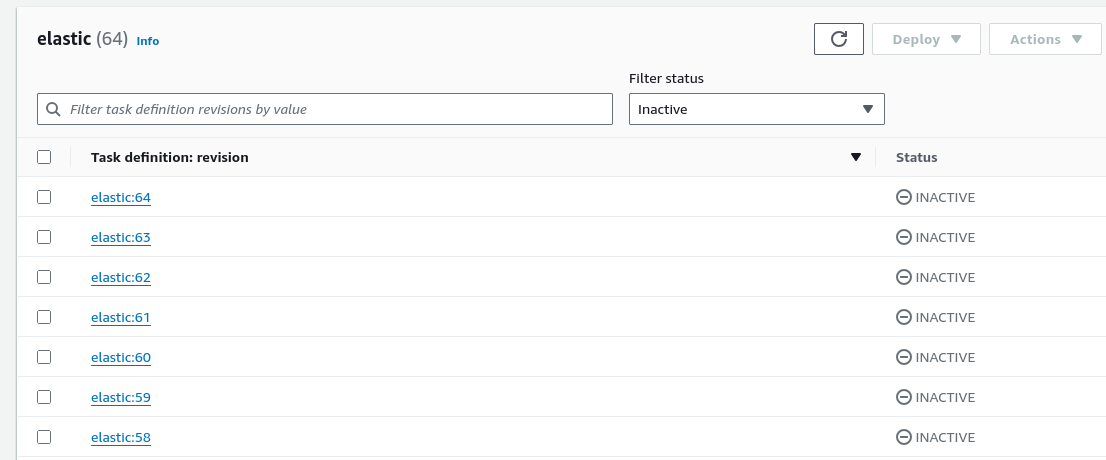
\includegraphics[width=\textwidth]{impl/definitions.png}
	\caption{Ejemplo de definciones de tareas de ECS en AWS}
	\label{fig:definitions}
\end{figure}

\begin{figure}[H]
	\centering
	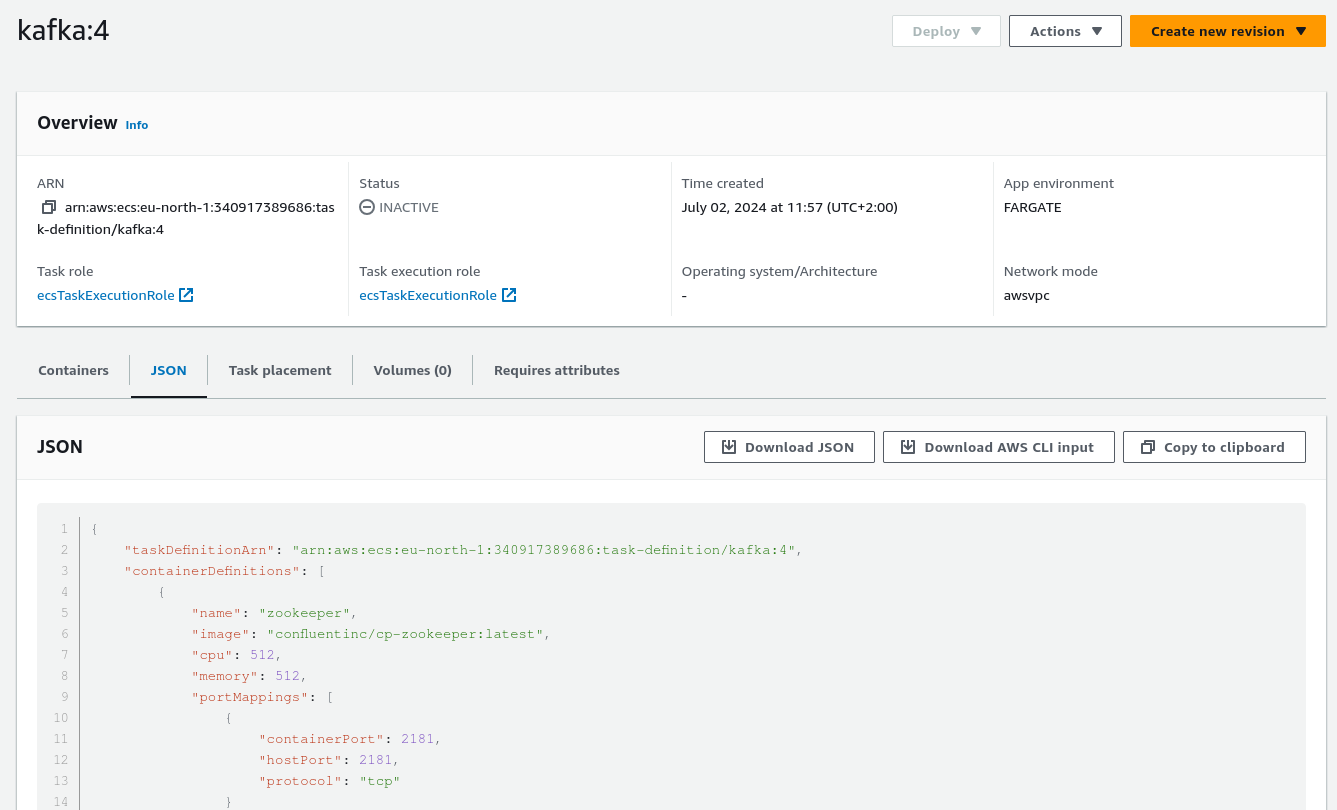
\includegraphics[width=\textwidth]{impl/ejemplo_definition.png}
	\caption{Ejemplo de definción de tarea (Kafka)}
	\label{fig:definition}
\end{figure}

Durante el desarrollo del despliegue, se utilizan las herramientas de
monitorización de AWS para comprobar el estado de los recursos y servicios
creados, y se realizan pruebas básicas de funcionamiento para asegurar que los
servicios se han desplegado correctamente. En la siguiente figura, se muestran
los logs de una tarea de ECS.

\begin{figure}[H]
	\centering
	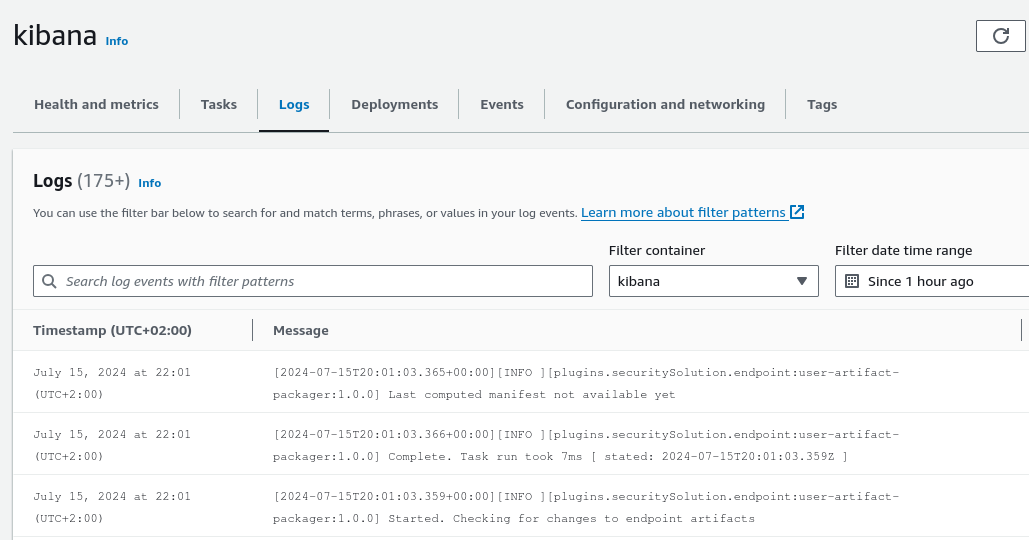
\includegraphics[width=\textwidth]{impl/task_logs.png}
	\caption{Ejemplo de logs de una tarea de ECS}
	\label{fig:task_logs}
\end{figure}

En la siguiente figura, se muestra el estado actual de todos los balanceadores
de carga, junto a más detalles como sus zonas de disponibilidad o el estado de
los nodos.

\begin{figure}[H]
	\centering
	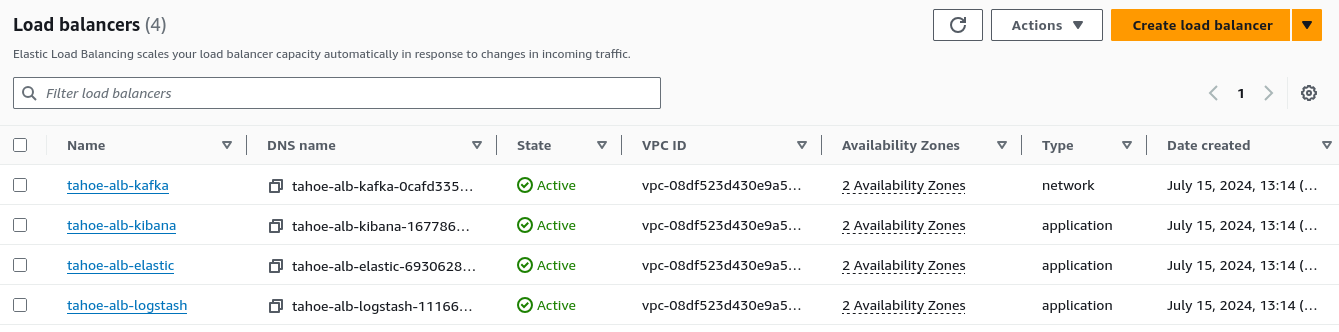
\includegraphics[width=\textwidth]{impl/estado_elb.png}
	\caption{Estado de los balanceadores de carga}
	\label{fig:estado_elb}
\end{figure}

Por último, en la siguiente figura, se muestra el estado de un despliegue de un
servicio, con información sobre el estado de los contenedores, la versión de la
imagen, la cantidad de tareas en ejecución y la cantidad de tareas deseadas.

\begin{figure}[H]
	\centering
	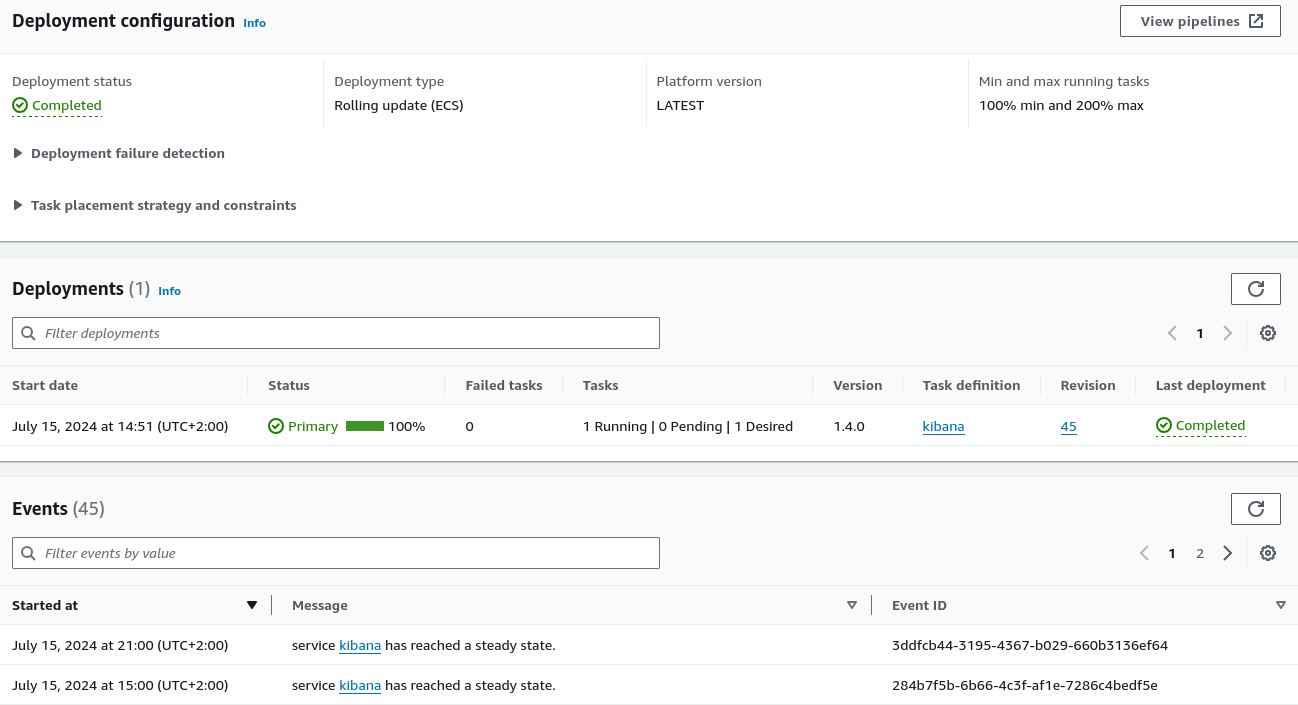
\includegraphics[width=\textwidth]{impl/deploy_state.png}
	\caption{Métricas de estado del despliegue de un servicio}
	\label{fig:deploy_state}
\end{figure}

Por supuesto, los propios servicios cuentan con sus herramientas de
monitorización básicas a las que se puede acceder a través del navegador (en
caso de que funcionen correctamente).

\begin{figure}[H]
	\centering
	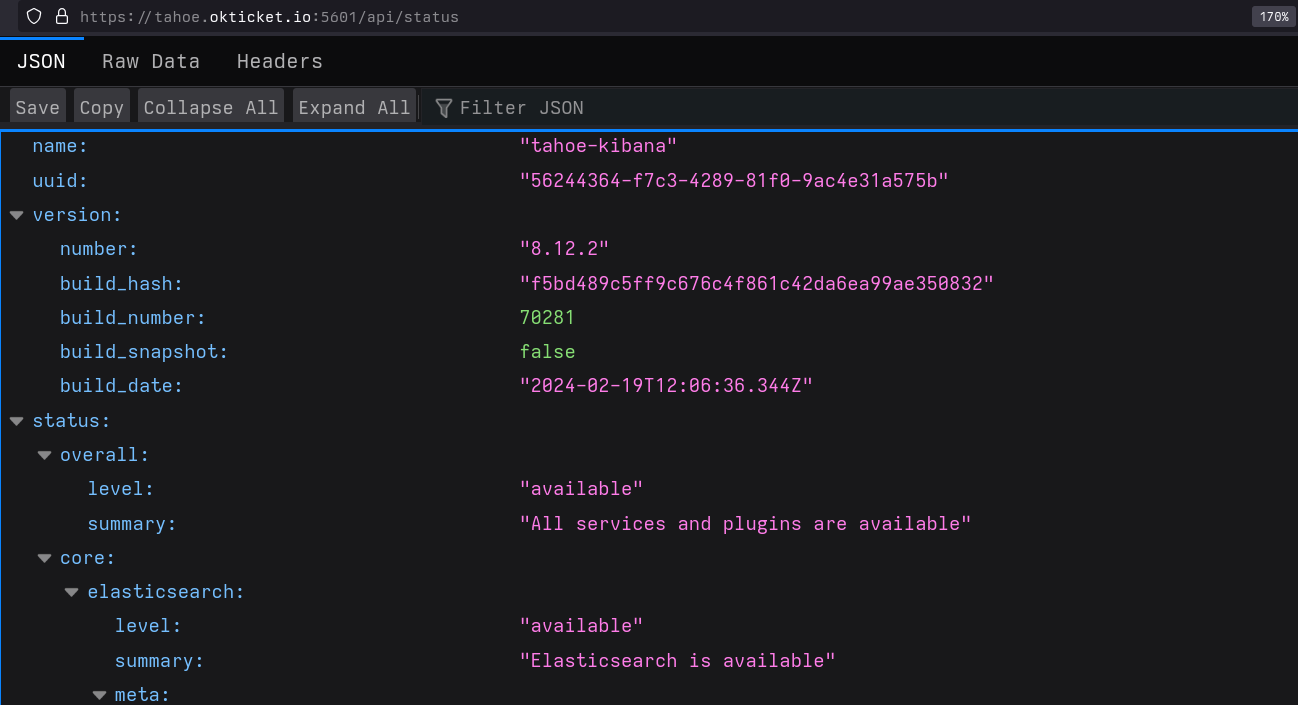
\includegraphics[width=\textwidth]{impl/kibana_status.png}
	\caption{Estado de Kibana}
	\label{fig:kibana_status}
\end{figure}

\begin{figure}[H]
	\centering
	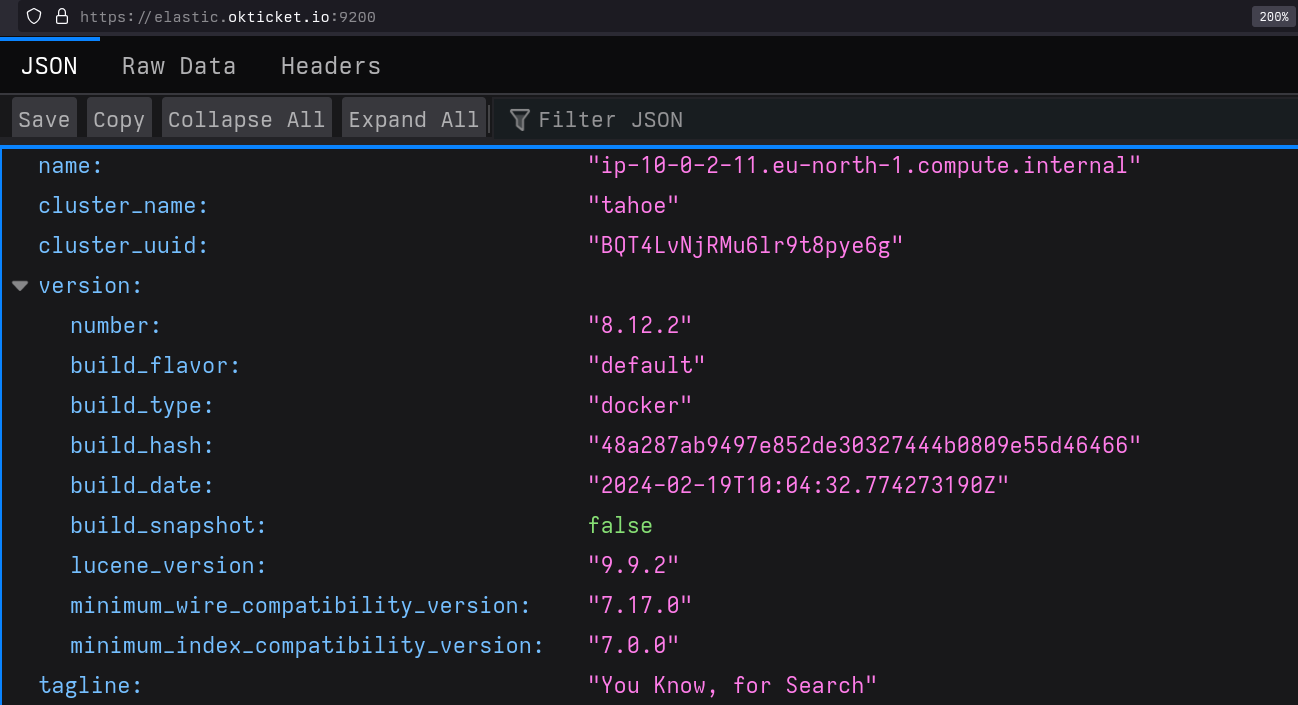
\includegraphics[width=\textwidth]{impl/elastic_status.png}
	\caption{Estado de Elasticsearch}
	\label{fig:elastic_status}
\end{figure}

Estas herramientas se utilizan para el desarrollo incremental y la comprobación
de que los servicios se despliegan correctamente, y se espera que, en la fase de
producción, no sea necesario su uso, puesto que se cuenta con herramientas de
monitorización más avanzadas y específicas para cada servicio.

\newpage{}
\subsection{Despliegue de la infraestructura}\label{subsec:impl_cloud_despliegue}
% TODO: desarrollar
% Aquí podría estar bien poner un diagrama de despliegue. Pero que se vea en el
% modelo que ese diagrama de despliegue no es el despliegue de tu proyecto.
% Es decir, el proyecto es crear un proceso de despliegue que hace un despliegue.
% Entonces que se vea que hay ese proceso y luego el diagrama de despliegue de lo
% que el proyecto permite desplegar


\newpage{}
\subsection{Explicación del código}\label{sec:impl_configuracion}
\emph{El código completo se encuentra en el anexo \fullref{anexo:cloud}.}

Los scripts de Terraform se dividen en varios archivos, cada uno de ellos con
una función específica, con el objetivo de facilitar la gestión y configuración
de los recursos y servicios. A continuación, se detallan dichos archivos y su
función en el proyecto.


\subsubsection{Recursos generales}
Como previamente descrito, la definción de los recursos generales se divide en
ficheros, cada uno de ellos con una función específica. A continuación, se
detallan dichos ficheros y su función en el proyecto.

\paragraph{Fichero principal}
El fichero principal de Terraform, \texttt{main.tf}, se encarga de las
configuraciones más esenciales o que no tienen cabida en otros ficheros, como
la definción de la región, el cluster, el grupo de logs o el bucket S3 de logs.

\textit{Ver código: \fullref{lst:main}}


\paragraph{Variables}
El fichero de variables (\texttt{variables.tf}) se encarga de la definición de
todas las variables necesarias para el despliegue de la infraestructura, como
nombres, regiones, versiones, puertos, etc., de manera que se puedan modificar y
reutilizar de manera sencilla a lo largo del resto de ficheros de definción.

También se definen contraseñas de manera aleatoria, para mejorar la seguridad
de los servicios.

\textit{Ver código: \fullref{lst:variables}}


\newpage{}
\paragraph{Salidas}
El fichero de salidas (\texttt{outputs.tf}) se encarga de la definición de las
salidas de Terraform, es decir, de las variables que se pueden consultar una vez
que se ha desplegado la infraestructura, como las direcciones URL de los servicios
o las contraseñas generadas alteatoriamente.

Un ejemplo de estas salidas se encuentra en la figura
\fullref{fig:terraform_output}.

\textit{Ver código: \fullref{lst:outputs}}


\paragraph{Volúmenes lógicos (EFS)}
El fichero de volúmenes lógicos (\texttt{efs.tf}) se encarga de la definción de
los volúmenes lógicos necesarios para la persistencia de los datos de los
servicios, como los datos de Elasticsearch o los logs de los servicios.

\textit{Ver código: \fullref{lst:efs}}


\paragraph{Roles, políticas y permisos (IAM)}
El fichero de roles, políticas y permisos (\texttt{iam.tf}) se encarga de la
definción de los roles y políticas necesarios para el correcto funcionamiento
de los servicios, como los roles de ejecución de tareas de ECS, los permisos
de acceso a los servicios de AWS o las políticas de acceso a los recursos.

\textit{Ver código: \fullref{lst:iam}}


\paragraph{Secretos}
El fichero de secretos (\texttt{secrets.tf}) se encarga de la definción de las
claves necesarias para el correcto funcionamiento de los servicios, como los
certificados de Elasticsearch o las claves de acceso a los servicios.

Estos secretos se almacenan en \textit{AWS Secrets Manager}, un servicio de AWS
que permite el almacenamiento seguro de información sensible, como contraseñas,
claves de acceso o certificados.

Los certificados se almacenan en formato \texttt{base64} para facilitar su
almacenamiento y evitar problemas de codificación en el paso de los mismos.

Se utilizan cadenas generadas aleatoriamente para evitar la exposición de
contraseñas y claves de acceso en el código.

\textit{Ver código: \fullref{lst:secrets}}


\paragraph{Redes}
El fichero de redes (\texttt{network.tf}) se encarga de la definción de los
elementos de red necesarios para la correcta comunicación entre los servicios y
su seguridad.

La lógica y arquitectura de red se explica en el apartado
\fullref{subsec:redes}, lo que facilita la definición de las redes en Terraform.

\textit{Ver código: \fullref{lst:network}}


\paragraph{Grupos de seguridad}
El fichero de grupos de seguridad (\texttt{security.tf}) se encarga de la
definción de los grupos de seguridad necesarios para la correcta comunicación
entre los servicios y su seguridad.

La lógica y arquitectura de seguridad se explica en el apartado
\fullref{subsec:seguridad}.

\textit{Ver código: \fullref{lst:security}}


\newpage{}
\subsubsection{Servicios de ELK}
Puesto que la estructura de definción de servicios en Terraform es similar para
todos los servicios, se analiza el más completo, Elasticsearch, para explicar el
funcionamiento y la lógica de los mismos.

Cada fichero de definción de servicios está separado en tres partes:
\begin{enumerate}
	\item \textbf{Definción de la tarea}, que contiene la configuración del
		contenedor al estilo de Docker (imagen, variables de entorno, volúmenes,
		etc.)
	\item \textbf{Definción del servicio}, que asigna la tarea al resto de la
		configuración del servicio.
	\item \textbf{Definción de recursos}, los necesarios para cada servicio:
		balanceadores de carga, \textit{listeners}, configuraciones DNS, etc.
\end{enumerate}

El código completo de los servicios se encuentra en el anexo \fullref{anexo:cloud}.

\paragraph{Definción de la tarea}
A continuación, se muestra un ejemplo de la definción de la tarea de Elastic:

\begin{lstlisting}[caption={Definción de la tarea de Elastic}, label={lst:elastic_task}]
	resource "aws_ecs_task_definition" "elastic" {
  family                   = "elastic"
  network_mode             = "awsvpc"
  requires_compatibilities = [var.launch_type]
  cpu                      = "2048"
  memory                   = "4096"
  execution_role_arn       = aws_iam_role.ecs_task_execution.arn
  task_role_arn            = aws_iam_role.ecs_task_execution.arn

  container_definitions = jsonencode([
    {
      name      = "es01"
      image     = "docker.elastic.co/elasticsearch/elasticsearch:${var.stack_version}"
      cpu       = 2048
      memory    = 4096
      essential = true
      environment = [
        { name = "cluster.name", value = var.cluster_name },
        { name = "xpack.security.enabled", value = "true" },
        { name = "xpack.security.http.ssl.enabled", value = "true" },
		<...>
      ]
      secrets = [
        {
          name      = "CA_CRT"
          valueFrom = "${aws_secretsmanager_secret.es_certs.arn}:ca.crt::"
        },
        {
          name      = "ES01_KEY"
          valueFrom = "${aws_secretsmanager_secret.es_certs.arn}:es01.key::"
        },
        <...>
      ]
      entrypoint = [
        "/bin/sh",
        "-c",
        <<-EOT
        #!/bin/bash
        set -e

        echo "Configurando credenciales..."
        mkdir -p /usr/share/elasticsearch/config/certs
        echo $CA_CRT | base64 -d > /usr/share/elasticsearch/config/certs/ca.crt
        <...>
        EOT
      ]
      # mountPoints = [
      #   {
      #     sourceVolume  = "elastic-data"
      #     containerPath = "/usr/share/elasticsearch/data"
      #     readOnly      = false
      #   }
      # ]
      portMappings = [
        {
          containerPort = var.elastic_port,
          hostPort      = var.elastic_port
        }
      ]
      logConfiguration = {
        logDriver = var.log_driver
        options = {
          "awslogs-group"         = var.log_group
          "awslogs-region"        = var.region
          "awslogs-stream-prefix" = "elastic"
        }
      }
      ulimits = [
        {
          name      = "memlock"
          softLimit = -1
          hardLimit = -1
        },
        {
          name      = "nofile"
          softLimit = 65536
          hardLimit = 65536
        }
      ]
    }
  ])

  volume {
    name = "elastic-data"
    efs_volume_configuration {
      file_system_id = aws_efs_file_system.elastic_data.id
      root_directory = "/"
    }
  }
}
\end{lstlisting}

Como se puede comprobar, pese a que la sintaxis de configuración es distinta,
la estructura de la misma es muy similar a aquella ya definida durante el
\fullref{sec:impl_local}, con similares configuraciones de entorno, mapeos de
puertos y volúmenes, y configuraciones de red. Ese es el objetivo del
planteamiento iterativo y de desarrollo incremental, que permite reutilizar
código y configuraciones ya definidas.

Al igual que en el desarrollo local, se obvia la configuración de los recursos
necesaria para la escalabilidad y replicación de los servicios, puesto que de
momento no se necesitan más que una instancia de cada servicio. Sin embargo,
esto no significa que no se pueda añadir de manera sencilla en un futuro, como
así lo demuestran, por ejemplo, la asignación de los servicios a volúmenes EFS.

A diferencia del desarrollo local, la preparación del servicio se realiza desde
la clave de configuración \texttt{entrypoint}, en lugar de requerir un segundo
contenedor de configuración.


\newpage{}
\paragraph{Definción del servicio}
A continuación, se detalla la definición del servicio de Elasticsearch:

\begin{lstlisting}[caption={Definción del servicio de Elastic}, label={lst:elastic_service}]
	resource "aws_ecs_service" "elastic" {
  name                   = "elastic"
  cluster                = aws_ecs_cluster.cluster.id
  task_definition        = aws_ecs_task_definition.elastic.arn
  desired_count          = 1
  launch_type            = var.launch_type
  enable_execute_command = true

  network_configuration {
    subnets          = [aws_subnet.private.id]
    security_groups  = [aws_security_group.elastic.id]
    assign_public_ip = true
  }

  load_balancer {
    target_group_arn = aws_lb_target_group.elastic.arn
    container_name   = "es01"
    container_port   = var.elastic_port
  }

  depends_on = [
    aws_lb_listener.elastic,
    aws_ecs_task_definition.elastic
  ]
}
\end{lstlisting}

La definción del servicio es mucho más breve que el resto de definiciones,
puesto que la mayoría de la configuración se realiza en la tarea. En este caso,
se asigna la tarea a un grupo de seguridad y a una subred privada, y se asigna
el servicio a un balanceador de carga, que se encargará de distribuir el tráfico
entre los contenedores.


\newpage{}
\paragraph{Definción de recursos}
Todos los recursos necesarios para el servicio, como el balanceador de carga, el
grupo de seguridad, el \textit{listener} o la configuración DNS, se definen a
continuación.

\begin{lstlisting}[caption={Definción de recursos de Elastic}, label={lst:elastic_resources}]
resource "aws_lb" "elastic" {
  name               = "tahoe-alb-elastic"
  internal           = false
  load_balancer_type = "application"
  security_groups    = [aws_security_group.elastic.id]
  subnets            = [aws_subnet.public_a.id, aws_subnet.public_b.id]

  access_logs {
    bucket  = aws_s3_bucket.access_logs.bucket
    prefix  = "elastic"
    enabled = true
  }
}

resource "aws_lb_target_group" "elastic" {
  name        = "tahoe-tg-elastic"
  port        = var.elastic_port
  protocol    = "HTTPS"
  vpc_id      = aws_vpc.main.id
  target_type = "ip"

  health_check {
    enabled             = true
    path                = "/"
    protocol            = "HTTPS"
    matcher             = "200"
    interval            = 300
    timeout             = 60
    healthy_threshold   = 2
    unhealthy_threshold = 5
    port                = tostring(var.elastic_port)
  }
}

resource "aws_lb_listener" "elastic" {
  load_balancer_arn = aws_lb.elastic.arn
  port              = var.elastic_port
  protocol          = "HTTPS"
  ssl_policy        = "ELBSecurityPolicy-2016-08"
  certificate_arn   = aws_acm_certificate.elastic.arn

  default_action {
    type             = "forward"
    target_group_arn = aws_lb_target_group.elastic.arn
  }
}

resource "aws_lb_listener" "elastic_https" {
  load_balancer_arn = aws_lb.elastic.arn
  port              = 443
  protocol          = "HTTPS"
  ssl_policy        = "ELBSecurityPolicy-2016-08"
  certificate_arn   = aws_acm_certificate.elastic.arn

  default_action {
    type = "redirect"
    redirect {
      port        = tostring(var.elastic_port)
      protocol    = "HTTPS"
      status_code = "HTTP_301"
    }
  }
}

resource "aws_acm_certificate" "elastic" {
  domain_name       = local.elastic_url
  validation_method = "DNS"

  lifecycle {
    create_before_destroy = true
  }
}

resource "aws_route53_record" "elastic" {
  zone_id = var.route53_zone_id
  name    = local.elastic_url
  type    = "A"

  alias {
    name                   = aws_lb.elastic.dns_name
    zone_id                = aws_lb.elastic.zone_id
    evaluate_target_health = false
  }
}

resource "aws_route53_record" "elastic_validation" {
  for_each = {
    for dvo in aws_acm_certificate.elastic.domain_validation_options : dvo.domain_name => {
      name   = dvo.resource_record_name
      record = dvo.resource_record_value
      type   = dvo.resource_record_type
    }
  }

  allow_overwrite = true
  name            = each.value.name
  records         = [each.value.record]
  ttl             = 60
  type            = each.value.type
  zone_id         = var.route53_zone_id
}

resource "aws_acm_certificate_validation" "elastic" {
  certificate_arn         = aws_acm_certificate.elastic.arn
  validation_record_fqdns = [for record in aws_route53_record.elastic_validation : record.fqdn]
}
\end{lstlisting}

Como para todos los servicios, se necesitan definir los recursos de red que
permitan acceder a los mismos, es decir:

\begin{itemize}
	\item Un balanceador de carga que distribuya el tráfico entre los
		contenedores de Elasticsearch.
	\item Un \textit{target group} que asigne los contenedores al balanceador de
		carga y permita la comprobación de la salud de los contenedores.
	\item \textit{Listeners} que permitan el acceso a los servicios desde el
		exterior o redirijan el tráfico a los contenedores dependiendo del
		puerto de conexión.
\end{itemize}

En el caso de Elastic (y el de otros servicios como Kibana), también se requiere
la configuración de un subdominio DNS y sus certificados pertinentes, para
facilitar el acceso a los servicios desde el exterior. Sin dichos subdominios,
la dirección URL de los servicios cambiaría cada vez que se desplegaran, lo que
dificultaría el acceso a los mismos. El tiempo de vida (\textit{TTL}) de estas
definiciones es de un minuto por defecto, lo que permite la actualización de
los certificados y la dirección URL de manera rápida y sencilla.
